\chapter{Safety and the PR2}
Point out which parts of the code are considered part of the hardware safety systems (e.g. joint current limits), 
and make it clear that changing them can cause problems.

Talk about guidelines for safe operation (e.g. is it OK in a normal lab environment?)

\chapter{PR2 hardware}

\section{What's in the box}
THe PR2 ships in 3 packages:

\begin{tabular}{| l | l |}
\hline      
  Main robot crate & Large wooden crate which contains the PR2 itself \\ \hline
  Accessory crate & Crate which contains accessory kit, tool kit, and robot base-station \\ \hline
  Calibration target & Large checkerboard for accurate calibration of stereo cameras \\ \hline
\end{tabular}

\subsection{PR2}
\subsection{Accessory kit}
\subsubsection{Wireless Joystick}
The PR2 ships with a bluetooth joystick for teleoperating the robot. The bluetooth joystick is a 
\href{http://www.sonystyle.com/webapp/wcs/stores/servlet/ProductDisplay?catalogId=10551&storeId=10151&langId=-1&productId=8198552921665411965#additionalImage1%22}{Sony DUALSHOCK®3} (Figure~\ref{fig:ps3joy}) 
wireless controller. It can be charged using any standard USB A to mini-B USB cable. For more information, see the 
\href{http://www.ros.org/wiki/ps3joy}{ps3joy} package at \href{http://www.ros.org}{ros.org}.

\begin{figure}[h]
\centering
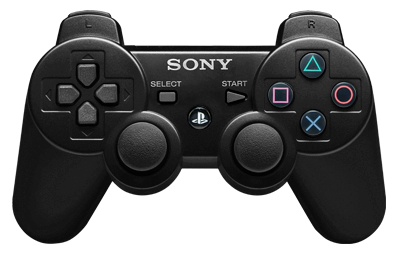
\includegraphics[scale=0.5]{ps3joy.png}
\caption{The PR2 bluetooth joystick.}
\label{fig:ps3joy}
\end{figure}

\subsubsection{Wireless run-stop}
\label{wirelessrunstop}
The PR2 comes with an \href{http://www.omnexcontrols.com/products/portable/t50.html}{OMNEX T50} 
wireless run-stop transmitter. When stopped or out of range, the wireless run-stop transmitter will halt the motors 
and put the power system in standby mode. 

\begin{figure}[h]
\centering
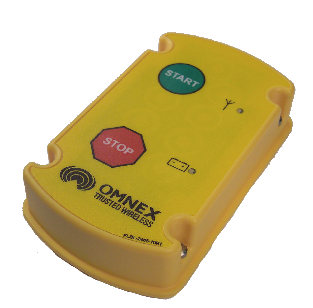
\includegraphics[width=150px]{run_stop.png}
\caption{The PR2 wireless run-stop.}
\label{fig:runstop}
\end{figure}

To start the run-stop, press the green start button (Figure~\ref{fig:runstop}); if this works properly, you will see a 
light flashing on the run-stop. While transmitting, the run-stop has a range of approximately 800 ft. The run-stop is 
powered by four AA batteries; the battery light will flash when the battery charge is low, which is an indication that 
you should change the batteries.

\TODO{Create and fill out subsection for every component of accessory kit}

\subsection{Toolkit}
\TODO{Include image of open toolkit, with callout labels to all tools by proper name}
\TODO{TBD: The robot toolkit is not yet fully defined}

\subsection{Calibration target}
The calibration target which ships with the robot will be is a checkerboard 1" thick and approximately 3 feet on a side.  This is the recommended calibration target to use for calibrating the intrinsics of the stereo cameras on the robot.  The robot ships with stereo cameras already calibrated, but you may need to re-calibrate occasionally as vibration and thermal effects change the parameters over time.

\subsection{Base-station computer}
\TODO{Include picture of base-station here}
The base-station computer ships without a monitor, keyboard, or mouse.  See section ??? for more information on how to configure your base-station.

\section{Mechanism}
PR2 is a 32-dof mobile manipulator with a mobile base, two arms, and a variety of sensors on a pan-tilt head.

\subsection{Robot Anatomy}

Kinematically speaking, the PR2 can be broken down into {\bf links} by individual degrees of freedoms.  Each {\bf link} consist of one
rigid body component that can be represented by a single collision model and a single lumped inertial property.
All links are interconnected together by {\bf joint} constraints in the form of revolute, prismatic or fixed {\bf joints}.
In this literature, a revolute joint without limits is also called a continuous joint.
In general, the entire PR2 mechanism is represented by a tree where each node is a {\bf link}
  and the edges connecting individual nodes are {\bf joints}.
In the tree representation of the PR2, each node (link) can be connected (via joints) to only one parent node but can have arbitrarily many child nodes.

A link without collision or inertial components is referred to as a {\bf frame}. Frames are always rigidly attached to parent links via fixed joints and cannot have children links.
A frame serves an important function of facilitating transform record keeping through our \href{http://www.ros.org/wiki/tf}{Transform and Frames Library (TF)}
  for propagating information such as reference coordinates of an optical image, origin of range sensor generated point cloud data or the reference pose for the grasp point of a gripper.

A CAD approximated kinematic and inertial description of the PR2 can be found
  in the \href{http://www.ros.org/wiki/pr2\_description}{pr2\_description} package.
This package uses a robot specific Extensible Markup Language (XML) and Document Object Model (DOM) representation
  called \href{http://www.ros.org/wiki/urdf}{Uniform Robot Description Format(URDF)} created here at Willow Garage.

Rather than diving into all 32 DOF's of the PR2 in detail right away, the next section examines the robot by its major components:  head, torso, arms, base and casters.
This overall breakdown of the PR2 robot is depicted in Figure~\ref{fig:pr2_basic_breakdown}.

\subsubsection{Head}
The PR2 head consists of two links: {\bf head\_pan\_link} and {\bf head\_tilt\_link}.  The {\bf head\_tilt\_link} is attached via a revolute joint called {\bf head\_tilt\_joint} to the {\bf head\_pan\_link}.
The {\bf head\_pan\_link} is attached to the PR2 torso ({\bf torso\_lift\_link}) by another revolute joint called the {\bf head\_pan\_joint}.

The individual head sensors are detailed separately in the section~\ref{subsec:pr2_sensors}

\subsubsection{Arms}
The PR2 arms can be further subdivided into shoulder, upper arm, forearm and gripper.  Each components is separately described in detail below:
\begin{itemize}
\item Shoulers
  \begin{itemize}
  \item {\bf l\_shoulder\_pan\_link} {\bf r\_shoulder\_pan\_link}
  \item {\bf l\_shoulder\_lift\_link} {\bf r\_shoulder\_lift\_link}
  \item {\bf l\_upper\_arm\_roll\_link} {\bf r\_upper\_arm\_roll\_link}
  \end{itemize}
\item Upper Arms
  \begin{itemize}
  \item {\bf l\_upper\_arm\_link} {\bf r\_upper\_arm\_link}
  \item {\bf l\_elbow\_flex\_link} {\bf r\_elbow\_flex\_link}
  \item {\bf l\_forearm\_roll\_link} {\bf r\_forearm\_roll\_link}
  \end{itemize}
\item Forearms
  \begin{itemize}
  \item {\bf l\_forearm\_link} {\bf r\_forearm\_link}
  \item {\bf l\_wrist\_flex\_link} {\bf r\_wrist\_flex\_link}
  \item {\bf l\_wrist\_roll\_link} {\bf r\_wrist\_roll\_link}
  \end{itemize}
\item Grippers
  \begin{itemize}
  \item {\bf l\_gripper\_palm\_link} {\bf r\_gripper\_palm\_link}
  \item {\bf l\_gripper\_l\_finger\_link} {\bf l\_gripper\_r\_finger\_link}
        {\bf r\_gripper\_l\_finger\_link} {\bf r\_gripper\_r\_finger\_link}
  \item {\bf l\_gripper\_l\_finger\_tip\_link} {\bf l\_gripper\_r\_finger\_tip\_link}
        {\bf r\_gripper\_l\_finger\_tip\_link} {\bf r\_gripper\_r\_finger\_tip\_link}
  \end{itemize}
\end{itemize}


\subsubsection{Torso}
The PR2 {\bf torso\_lift\_link} refers to the torso part of the PR2 that moves up and down with the elevator actuator.

\subsubsection{Base}
The PR2 {\bf base\_link} is the lower part of the PR2 body, housing the PR2 computers and is also rigidly attached to the base Hokuyo laser scanner.

\subsubsection{Casters}
The PR2 has 4 caster units.  Each caster contains one actuated steering degree of freedom and two individually actuated wheels.

\subsubsection{Home Pose}
In order to describe the PR2 robot pose and joint positions in a consistent manner, a {\bf home pose} of the robot has been defined.  The {\bf home pose} is described in detail in section~\ref{sec:pr2_coordinate_system}.

\subsubsection{Sensors}
\label{subsec:pr2_sensors}
Details of the PR2 sensors are described here.
The PR2 contains the following sensors:
\begin{itemize}
\item Image Sensors
  \begin{itemize}
  \item Dual Stereo Cameras
    \begin{itemize}
    \item Narrow Stereo Camera Pair
    \item Wide Stereo Camera Pair
    \end{itemize}
  \item Prosilica Camera
  \item Forearm Cameras
  \end{itemize}
\item Range Sensors
  \begin{itemize}
  \item Tilting Hokuyo Laser Scanner
  \item Base Hokuyo Laser Scanner
  \end{itemize}
\item Accelerometers
  \begin{itemize}
  \item IMU
  \item Gripper Palm Mounted Accelerometers
  \end{itemize}
\end{itemize}


\subsubsection{PR2 Coordinate System}
\label{sec:pr2_coordinate_system}
The reference {\bf home pose} of the PR2 robot is defined as the robot pose with all the joint angles at zero,
with the PR2 robot facing the positive x-direction, positive z-axis pointing upwards and positive y-axis pointing to the {\it robot-left} (see Figure~\ref{fig:pr2_home_pose}).

\begin{figure}[!h]
\centering
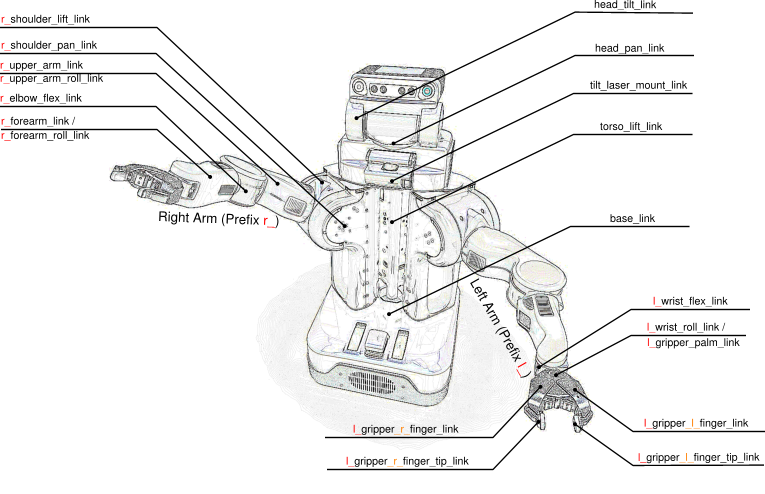
\includegraphics[scale=0.3]{urdf_links.png}
\caption{The PR2 URDF Link Naming Scheme.}
\label{fig:urdf_link_names}
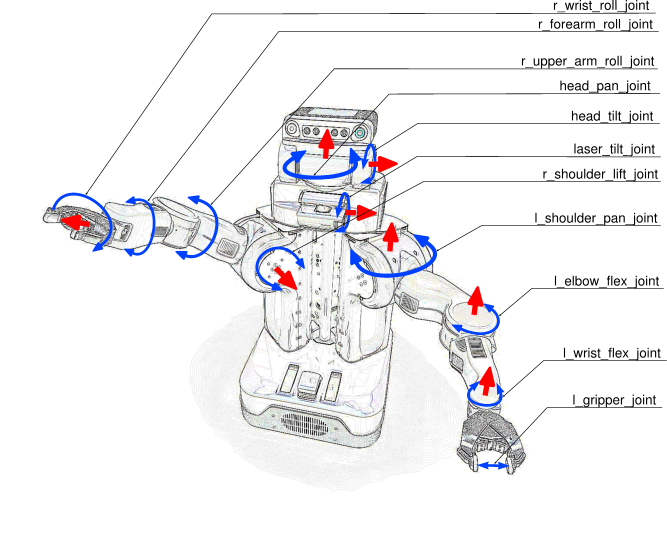
\includegraphics[scale=0.3]{urdf_joints.png}
\caption{The PR2 URDF Joints Naming Scheme.}
\label{fig:urdf_joints}
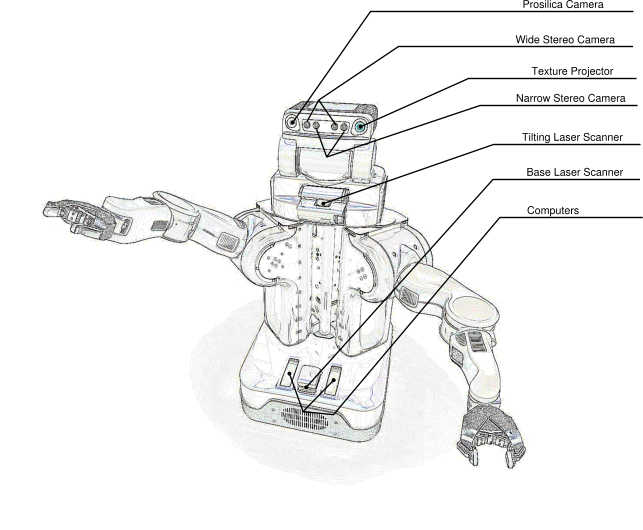
\includegraphics[scale=0.3]{urdf_sensors.png}
\caption{The PR2 Sensors.}
\label{fig:urdf_sensor}
\end{figure}

\subsection{Drivetrains}
The PR2 drivetrains have been designed to be low inertia and
backdrivable with minimal backlash. There are three types of
drivetrains on the PR2, gear drives, belt drives, and lead screw
drives.  

\subsubsection{Belt Drives}
The most common drivetrain on the PR2 is the belt drive.  

The typical link drivetrain is a DC motor with attached encoder.  It
runs through a planetary gearbox then is attached to a belt
drive. These drivetrains are fully backdriveable and have low
backlash.

\TODO{Belt drive Diagram}

The following motors use belt drives as described above:
\begin{itemize}
\item Caster Wheel
\item Caster Turret
\item Head Tilt
\item Head Pan
\subitem Note: The gearbox is replaced by gears, with the encoder on the mechanism side of the gears.  
\item Shoulder Pan
\item Shoulder Lift
\item Upper Arm Roll
\item Upper Arm Flex
\subitem Note: There is an additional 90 degree bevel gear pair on this joint between the gearbox and the belt drive. 
\item Laser Tilt
\subitem Note: There is no gearbox, there is a flex coupler in it's place.  And the encoder is on the mechanism side of the flex coupler.
\end{itemize}


\subsubsection{Gear Drives}
The wrist, head pan and forearm roll use 
\paragraph{Wrist }
The wrist utilized a differential drive between 
\TODO {wrist diagram}

\paragraph{Forearm roll }
The forearm roll has a traditional encoder, motor, gearbox assembly
with a pinion gear attached to the output shaft.  The pinion gear
directly drives a nylon gear built into the forearm body.

\subsubsection{Lead Screw Drives}
There are two drive trains which use lead screws as their primary
method of movement, the torso lift and gripper.  

\paragraph{Torso Lift }
The torso lift is driven by a vertical lead screw.  The motor is
augmented by a gas spring vertically such that the motor only needs to
lift a portion of the weight of the torso.  The torso is also mounted
such that the lift mechanism cannot pull downward. \TODO{check this is still true} 

\paragraph{Gripper }
The gripper is a pair of 4 bar linkages which are coupled through a
gearing on one of the piviots.  The mechanism is actuated using a lead
screw between the two fourbar linkages. Between the actuator and the
gearing the movement of the grippers is limited to a single degree of
freedom.

The gripper is backdriveable when off, however challenging.
Backdriving the gripper when torque is applied is very hard, but
possible.

\subsubsection{Possible Errors}
\paragraph{Fault Conditions}
\paragraph{Observed failures during testing}
\begin{itemize}
\item Belt broken \TODO {document counterbalance failure??}
\item Stripped belt teeth
\item Loose set screw
\end{itemize}
\paragraph{Running Errors}
There has been no measured hysteresis or backlash in the drivetrains
except in the two forms below.  \TODO{verify with vijay}

\paragraph{Belt Stretch}
This is unavoidable.  So far it has not been enough to effect usage.
It is large enough to be measured by the calibration.
\paragraph{Encoder Noise}
This is unavoidable.  It usually manifests itself as a jitter in the
velocity.  It can be filtered out to some extent, but not too much for
it will cause lag.



Discuss the drive-train approach, how/why things work, what types of errors we expect to see and don't expect to see

\subsection{Motion control}


\begin{figure}[h]
\centering
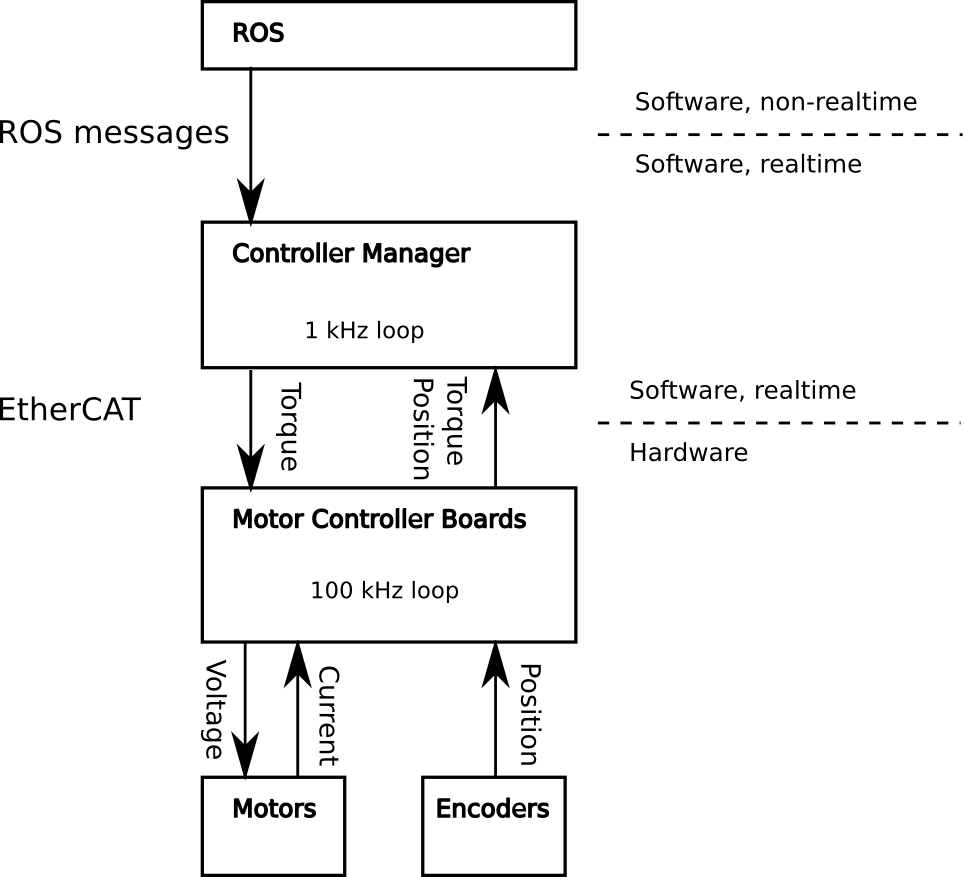
\includegraphics[width=290px]{images/mechanism_control.png}
\caption{Motion control layout.}
\label{fig:motion_control}
\end{figure}


\subsubsection{Motor controller boards}
Each motor/encoder on the PR2 has its dedicated \emph{Motor Controller
  Board} (MCB). The MCB detects and counts transitions in the encoder
signal, measures the current the motor is using, and commands the
voltage going to the motor. Each MCB runs a PI-control loop to control
the motor current to a desired value, by commanding the motor
voltage. This control loop is executed at 100~kHz on an FPGA.  A
shared etherCAT link allows all MCB's in the PR2 to communicate with
the main computers.

\subsubsection{Controller manager}
The \emph{Controller Manager} (CM) is the lowest level software
component that directly talks to the MCB's. The CM runs in a hard
realtime process and is guaranteed to be executed at 1~kHz. This means
the CM sends desired motor torques to the MCB's every milisecond, and
receives measured motor torques and positions in the same milisecond.

The CM has a dynamic plugin loading mechanism that allows controller
algorithms to get inserted and executed inside the 1~kHz realtime
loop.


\subsection{Mechanical specs}

Before undertaking any new or risky operations with your PR2, please consult these mechanical specifications. Do not operate the PR2 outside of these specifications. If you have any questions about your PR2's specifications, please contact Willow Garage Support.

\subsubsection{Environmental specs}

The PR2 is an indoor, household robot. Operating outside this type of environment could cause damage to the PR2, or injury or death to operators.

\paragraph{Water}

The PR2 has not been tested for any type of contact with water or any other liquid. Under no circumstances should the PR2 come in contact with water from rain, mist, ground water (puddles) or liquid handling. Water contact can cause damage to the electrical circuitry and the mechanism.

\paragraph{Temperature and Humidity}

Temperature testing of the PR2 has allowed the unit to run between 15 and 35C. Temperatures outside of this range can cause malfunctions in the PR2 power system and instruments. The PR2 has been tested in high humidity, but under no circumstances should condensation be allowed to form on the vehicle.

\paragraph{Drive Surface}

The drive surface of the PR2 must be capable of supporting the entire weight of the PR2, about 450 pounds (220 kgs). If the surface is too soft, the PR2 can get stuck and fail to drive. A commercial carpet or tile is recommended. 

\paragraph{Incline Surface}

The PR2 is ready for ADA compatible ramps, which specifies a 1/12 slope. Ramps that are steeper than 1/12 slope are unsafe and may be a tip over hazard.

\paragraph{Other Environmental Specs}

\begin{itemize}
\item UV exposure should be minimized. UV radiation can damage the PR2's skin
\item Dust and dirt can clog air filters
\end{itemize}

\subsubsection{Forces and torques}

Joint position, velocity, and force limits are implemented in the PR2's URDF file, in the ``/etc/ros/urdf/robot.xml" file on your PR2. These joint limits control the range of travel of the mechanism, the allowable velocity to prevent overtravel. These limits are enforced by pr2\_controller\_manager, and are designed to prevent poorly designed controllers from damaging the PR2 and harming operators. 



The limits below are from the PR2 URDF file. If a velocity or torque limit is not specified, no value is enforced by pr2\_controller\_manager.

\begin{tabular}{l*{2}{c}}
Joint  & Velocity (rad/s or m/s) & Torque (Nm or N) \\
\hline \hline
$\ast$\_caster\_rotation\_joint        & -     & -  \\
$\ast$\_caster\_wheel\_$\ast$\_joint   & -     & -  \\
torso\_lift\_joint                     & 0.013 & 10000 \\
laser\_tilt\_joint                     & 10.00 & 0.65  \\
head\_pan\_joint                       & 6.00  & 2.65  \\
head\_tilt\_joint                      & 5.00  & 15.00 \\
$\ast$\_shoulder\_pan\_joint           & 2.10  & 30.00 \\
$\ast$\_shoulder\_lift\_joint          & 2.10  & 30.00 \\
$\ast$\_upper\_arm\_roll\_joint        & 3.27  & 30.00 \\
$\ast$\_elbow\_flex\_joint             & 3.30  & 30.00 \\
$\ast$\_forearm\_roll\_joint           & 3.60  & 30.00 \\
$\ast$\_wrist\_flex\_joint             & 3.10  & 10.00 \\
$\ast$\_wrist\_roll\_joint             & 3.60  & 10.00 \\
$\ast$\_gripper\_joint                 & 0.20  & 1000  \\
\end{tabular}

The PR2 motor controller boards (MCB's) will not allow a current command greater than the maximum continuous current specified for the joint's actuator. This means that maximum joint effort may be lower than the maximum effort specified above. Below are the actuators for each joint (Maxon part number), and their maximum allowable commanded current. 

\begin{tabular}{ll*{2}{c}}
Joint  & Motor & Power (W) & Max Current \\
\hline \hline
$\ast$\_caster\_rotation\_joint       & 236672 & 20  & 0.655 \\
$\ast$\_caster\_wheel\_$\ast$\_joint  & 236672 & 20  & 0.655 \\
torso\_lift\_joint                    & 148877 & 150 & 3.12  \\
laser\_tilt\_joint                    & 310009 & 60  & 1.72  \\
head\_pan\_joint                      & 310009 & 60  & 1.72  \\
head\_tilt\_joint                     & 310009 & 60  & 1.72  \\
$\ast$\_shoulder\_pan\_joint          & 148877 & 150 & 3.12  \\
$\ast$\_shoulder\_lift\_joint         & 148877 & 150 & 3.12  \\
$\ast$\_upper\_arm\_roll\_joint       & 148877 & 150 & 3.12  \\
$\ast$\_elbow\_flex\_joint            & 148877 & 150 & 3.12  \\
$\ast$\_forearm\_roll\_joint          & 310009 & 60  & 1.72  \\
$\ast$\_wrist\_flex\_joint            & 310009 & 60  & 1.72  \\
$\ast$\_wrist\_roll\_joint            & 310009 & 60  & 1.72  \\
$\ast$\_gripper\_joint                & 222057 & 11  & 0.204 \\
\end{tabular}

More information about each actuator may be found in Maxon datasheets.

\subsubsection{Joint Limits and Types}

The position limits for the PR2 are specified below. These ``hard limits" are the maximum travel for the mechanism. 

\begin{tabular}{ll*{2}{c}}
Joint  & Type  & Limit (+) & Limit (-) \\
\hline \hline
$\ast$\_caster\_rotation\_joint        & continuous & -            & - \\
$\ast$\_caster\_wheel\_$\ast$\_joint   & continuous & -            & - \\
torso\_lift\_joint                     & prismatic  & 310 mm       & 0 mm \\
laser\_tilt\_joint                     & revolute   & 85$^\circ$   & 45$^\circ$ \\
head\_pan\_joint                       & revolute   & 168$^\circ$  & 168$^\circ$  \\
head\_tilt\_joint                      & revolute   & 60$^\circ$   & 30$^\circ$  \\
r\_shoulder\_pan\_joint                 & revolute   & 40$^\circ$   & 130$^\circ$  \\
l\_shoulder\_pan\_joint                 & revolute   & 130$^\circ$  & -40$^\circ$  \\
$\ast$\_shoulder\_lift\_joint          & revolute   & 80$^\circ$   & 30$^\circ$  \\
r\_upper\_arm\_roll\_joint              & revolute   & 44$^\circ$   & -224$^\circ$  \\
l\_upper\_arm\_roll\_joint              & revolute   & 224$^\circ$  & -44$^\circ$  \\
$\ast$\_elbow\_flex\_joint             & revolute   & 133$^\circ$  & 0$^\circ$  \\
$\ast$\_forearm\_roll\_joint           & continuous & -            & - \\
$\ast$\_wrist\_flex\_joint             & revolute   & 130$^\circ$  & 0$^\circ$  \\
$\ast$\_wrist\_roll\_joint             & continuous & -            & - \\
$\ast$\_gripper\_joint                 & prismatic  & 86 mm        & 0 mm \\
\end{tabular}

\subsubsection{Modifying Joint Limits}

On the PR2, ``soft limits" stop the joints from reaching the full range of motion to prevent damage to the mechanism. These soft limits, similar to a virual spring, are specified in the robot's URDF file. For an explanation of their implementation, see http://www.ros.org/wiki/pr2\_controller\_manager/safety\_limits.

The soft limits have been carefully implemented and validated by Willow Garage. Under no circumstances should they be changed without prior written authorization by Willow Garage Safety. Unauthorized and unvalidated modification of these limits could cause mechanism damage and injury or death to PR2 operators. 

Changing maximum allowable effort or maximum actuator current could cause serious damage to the PR2 and injury or death to operators. 

\section{Sensors}
The PR2 has a variety of sensors spread out over it's body:\\\\
\begin{overpic}[scale=0.45]{sensors.png}
\put(46.9,50.9){\href{http://www.ros.org/wiki/prosilica_camera}{
\includegraphics[scale=0.45]{sensors_prosilica.png}}}
\put(49,51){\href{http://www.ros.org/wiki/wge100_camera}{
\includegraphics[scale=0.45]{sensor_camera.png}}}
\put(55.3,50.9){\href{http://www.ros.org/wiki/}{
\includegraphics[scale=0.45]{sensors_projector.png}}}
\put(47.6,43.7){\href{http://www.ros.org/wiki/hokuyo_node}{
\includegraphics[scale=0.45]{sensors_tilt_laser.png}}}
\put(43.05,19.9){\href{http://www.ros.org/wiki/hokuyo_node}{
\includegraphics[scale=0.45]{sensors_base_laser.png}}}
\put(61.8,23.6){\href{http://www.ros.org/wiki/wge100_camera}{
\includegraphics[scale=0.45]{sensors_r_forearm.png}}}
\put(26.4,30.9){\href{http://www.ros.org/wiki/wge100_camera}{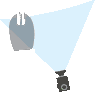
\includegraphics[scale=0.45]{sensors_l_forearm.png}}}
\end{overpic}

\subsection{Base Laser}
The base laser of the PR2 is \href{http://www.hokuyo-aut.jp/02sensor/07scanner/utm_30lx.html}{Hokuyo Top-URG (UTM-30LX)} 
scanning range finder that is located on PR2's base. This laser has a 30 m and 270$^\circ$ scanning range. For more information, 
see the \href{http://www.ros.org/wiki/hokuyo_node}{hokuyo\_node} package at \href{http://www.ros.org}{ros.org}.

\subsection{Tilting Laser}
\label{tilting laser}
In addition to the base laser, the PR2 has a \href{http://www.hokuyo-aut.jp/02sensor/07scanner/utm_30lx.html}{Hokuyo Top-URG (UTM-30LX)}
mounted on a tilting platform that is located just below the pan-tilt head. The tilting platform can sweep the scanning 
laser through 135$^\circ$ ($+90^\circ$ and $-45^\circ$ from level) and can be controlled using the
default laser\_tilt\_controller. For more information, see the \href{http://www.ros.org/wiki/hokuyo_node}{hokuyo\_node} 
and \href{http://www.ros.org/wiki/pr2_default_controllers}{pr2\_default\_controllers} packages at \href{http://www.ros.org}{ros.org}.

\subsection{Head Cameras}
The PR2 pan-tilt head has three cameras and a textured light projector:
\begin{description}
\label{stereo camera}
\item[Wide Stereo Camera]
The wide stereo camera of the PR2 is part of the dual stereo pair and is a 100Mb color ethernet camera. The wide stereo 
uses the \href{http://www.aptina.com/products/image_sensors/mt9v032c12stc/#overview}{Aptina MT9V032C12STC} imager chip
and has a maximum resolution of 752 x 480 pixels at 15 fps. The camera has a field of view (FOV) of approximately 
$90^\circ$ and a 2.5mm F2.5 \href{http://www.mars-cam.com/lenses/ccd_cmos/Technology%20Report(V-4402.5-2.5-HR).pdf}{Marshall V-4402.5-2.5-HR} 
lens. For more information, see the \href{http://www.ros.org/wiki/wge100_camera}{TODO} package
at \href{http://www.ros.org}{ros.org}.

\item[Narrow Stereo Camera]
The narrow stereo camera of the PR2 is part of the dual stereo pair and is a 100Mb monchrome ethernet camera. 
The narrow stereo uses the \href{http://www.aptina.com/products/image_sensors/mt9v032c12stm/#overview}{Aptina MT9V032C12STM} 
imager chip and has a max resolution of 752 x 480 pixels at 15 fps. The camera has a FOV of approximately $55^\circ$ and 
a 5.6mm F2.0  \href{http://www.mars-cam.com/lenses/ccd_cmos/Technology%20Report(V-4405.6-2.0-HR).pdf}{Marshall V-4405.6-2.0-HR}
lens. For more information, see the \href{http://www.ros.org/wiki/wge100_camera}{TODO} package
at \href{http://www.ros.org}{ros.org}.

\item[Gigabit Ethernet Camera]
\label{ethernet camera}
The PR2 has a gigabit ethernet camera located to the left of the dual stereo pair on the pan-tilt head. 
The gigabit ethernet camera is a \href{http://www.prosilica.com/products/gc2450.html}{Prosilica GC2450C},  
which uses the Sony ICX-625AQ imager chip and has a maximum resolution of 2448 x 2050 pixels at 15 fps. 
Additionally, the gigabit ethernet camera has a 8mm F1.4-F16 \href{http://www.kowascope.com/frontend/proddetail.asp?pn=LM8JC&co=10000348}{Kowa LM8JC} 
lens. For more information, see the \href{http://www.ros.org/wiki/prosilica_camera}{prosilica\_camera} 
package at \href{http://www.ros.org}{ros.org}.

\item[Textured Light Projector]
\label{texture projector}
The PR2 has a textured light projector located to the (robot's) left of the dual stereo pair on the pan-tilt head. 
The projector has a FOV of approximately $55^\circ$ and a 5.6mm F2.0 \href{http://www.kowascope.com/frontend/proddetail.asp?pn=LM12JC&co=10000348}{Kowa LM12JC} 
lens.  For more information, see the \href{http://www.ros.org/wiki/TODO}{TODO} package at \href{http://www.ros.org}{ros.org}.

\end{description}

\subsection{Forearm cameras}
Each forearm of the PR2 is equipped with a 12V 100Mb color ethernet camera. The forearm camera uses the 
\href{http://www.aptina.com/products/image_sensors/mt9v032c12stc/#overview}{Aptina MT9V032C12STC}  imager chip
and has a maximum resolution of 752 x 480 pixels at 15 fps. Additionally, the forearm camera has a 2.5mm F2.0 lens.  
For more information, see the \href{http://www.ros.org/wiki/wge100_camera}{wge100\_camera} package
at \href{http://www.ros.org}{ros.org}.

\subsection{Gripper Sensors}
\begin{description}

\item[Accelerometer]
The gripper of the PR2 is equipped with a \href{http://www.bosch-sensortec.com/content/language1/html/3474.htm}{Bosch BMA150} 
digital triaxal accelerometer. The measurement range ($\pm$2g, $\pm$4g, or $\pm$8g) and bandwidth (25Hz - 1500Hz) 
of the accelerometer can be selected in software. For more information, see the \href{http://www.ros.org/wiki/wge100_camera}{TODO} 
package at \href{http://www.ros.org}{ros.org}.

\item[Fingertip Pressure Sensors]
The default fingertips of the PR2 are sturdy aluminum blocks with non-slip 
rubber covers, for added friction and compliance in grasping.  However, the 
aluminum tips can be swapped out for an (included) set of RoboTouch tactile 
sensing pads made by Pressure Profile Systems, each with 22 tactile sensing 
elements: 15 in a 5x3 array on the front surface, 2 on top, 2 on each side, 
and 1 in back, near the top.  Each tactile element has a pressure range of 
0-30 psi (0-205 kPa) and sensitivity of 0.1 psi (0.7 kPa).  The sensors 
connect to the robot via an SPI ribbon cable and two screws, and have a 
maximum scan rate of 35 Hz.

The tactile sensors are highly fragile when not protected by the rubber 
covering, and so care should be taken not to damage the rubber covering when 
the tactile sensors are being used on the robot.  For more information, 
see the \href{http://www.ros.org/wiki/fingertip\_pressure}{fingertip\_pressure} package at \href{http://ros.org}{ros.org}.

\item[Calibration LED]

\end{description}

\subsection{Inertial measurement unit}
The PR2 has an inertial measurement unit (IMU) located next to the tilting laser. The IMU is a 
\href{http://www.microstrain.com/3dm-gx2.aspx}{MicroStrain Inertial-Link 3DM-GX2} which has an 
accelerometer range of $\pm$5g and a gyro range of $300^\circ/s$. For more information, see 
the \href{http://www.ros.org/wiki/microstrain_3dmgx2_imu}{microstrain\_3dmgx2\_imu} package 
at \href{http://www.ros.org}{ros.org}.

\subsection{Speaker}
The PR2 has one \href{http://www.logitech.com/index.cfm/speakers_audio/home_pc_speakers/devices/199&cl=us,en}{Logitech V20 notebook speaker} 
that is located under the pan-tilt head next to the tilting laser. For more information, 
see the \href{http://www.ros.org/wiki/sound_play}{sound\_play} package at \href{http://www.ros.org}{ros.org}.

\section{Power system}
\subsection{Overview}
The PR2 has a Lithium-ion (Li-ion) battery system that is charged off of 120V wall current and provides power the computers, motors, and sensors in the system.  Power distribution is controlled by the {\it Power Board}, which communicates over Ethernet.
\subsection{Power Busses}
The robot has several internal power busses:
\begin{description}
\item[120v] The robot has a 3-prong IEC320 plug in the back of the base, which is connected through a circuit breaker to the inputs of the four AC-DC converters that are used to charge the battery packs.  The system is designed to pull up to 15A, so it is fine to plug the robot in to any 15A wall socket, but you should make sure there are no other devices which draw significant power on the same circuit (e.g., computers or heaters).
%LT: Ideally, add image of back panel once we have the PR2 betas done w/ Ryan's stickers on that panel.
\item[Motor Power Bus] The motor controllers are fed from circuit breakers on the power board. The motor power bus can be in one of three states.  When enabled, they provide a direct connection to the unregulated battery power, which ranges from 52V when the batteries are fully discharged up to 72V when connected to wall power.  When the motors are in standby mode, the power board provides a low-power 18V supply that is used for communication and maintaing encoder position counts.  When disabled (e.g., in the event of a major power-system problem or if manually disabled), these circuit-breakers will also shut off without cutting power to the computers or sensors.  There are three independent motor power busses - left arm, right arm, and base/head, which can be monitored 
\item[12V system bus]
12V power for sensors that is provided by the power board.  This is also the recommended source of power for user modifications.
%LT: What do you mean by "user modifications?"
\item[12V computer power]
12V power for computers that is provided by the power board.
\end{description}
\subsection{Batteries}
The battery system has four battery bays comprised of four \href{http://www.oceanserver-store.com/18.html}{Ocean Server BA95HC-FL}
14.4V Li-ion batteries, a \href{http://www.v-infinity.com/adtemplate_child.asp?c=710918&p=903285&catky=764537&subcatky1=46887&subcatky2=320934}{V-INFINITY VF-S320-18A-CF}
18V AC-DC Power Supply, and a \href{http://www.oceanserver-store.com/xpmibamamo.html}{Ocean Server XP-04SRW} four-channel high 
current battery controller. This provides the PR2 with approximately two hours of countinous operation after a full recharge. 
For more information, see the \href{http://www.ros.org/wiki/ocean\_server}{ocean\_server} package at \href{http://www.ros.org}{ros.org}.

\subsection{Power board}

\subsection{Getting Power for sensors}
The electrical system in the robot is comprised of two primary systems. One operates from the batteries and is an unregulated voltage. The second bus provides a well regulated 12V supply. The regulated 12V supply is the only supply designed for additions and expansion. This 12V supply is essentially always on once the Power board completes a self test. It is also monitored for undervoltage conditions and is fairly robust.


A few limitations should be followed when adding loads to the 12V user supply. This supply is already supporting the 2 Hokuyo scanners, 2 ethernet switches, the wireless AP and the E-stop receiver. Considering the loads and the supplies capabilities with some headroom this leaves 5A for expansion.\\

{\bf 5A limit on 12V expansion}\\

Access to the 12V accessory bus is available in several locations:\\

Inside the top head assembly.\\

{\bf insert picture}\\


In the upper back.\\

{\bf insert picture}\\


In the lower back, directly connecting to the power board.\\

{\bf insert picture}\\

Before something is connected to this bus, strongly consider if hot plugging is safe. If you are uncertain, the safest choice is to shut the power system off completely.\\

All 12V connectors in the robot use the same connector, a 2x1 Molex Mini-Fit Jr. The mating connector part number is {\bf 39-01-3022} or from Digikey {\bf WM1021-ND}. Pin one is negative and pin 2 is positive. Pin 2 is the pin closest to the latch.
